\chapter{Introduction}

The Standard Model (SM) of particle physics is the theory that best decribes our current understanding of fundamental particles and their interactions. It describes a broad range of phenomena and makes a plethora predictions, many of which have been confirmed via measurement to great degrees of accuracy \cite{PhysRevD.110.030001}. A noteable feature of the SM is the Brout-Englert-Higgs (BEH) mechanism \cite{Higgs}\cite{EnglertBrout}, which predicts the existance of a Brout-Englert-Higgs (or often simply Higgs) boson. The EBH mechanism is considered a central part of the SM as it provides a unique mechanism by which SM particles may acquire mass through their interaction with the Higgs boson. As such, the experimental discovery of a Higgs-like scalar boson in 2012 \cite{HiggsDiscovery2012CMS}\cite{HiggsDiscovery2012ATLAS} was a major milestone in particle physics. Since this discovery, a significant open question that remains is whether this particle indeed behaves entirely in an SM-like way. Measuring the exact properties of the discovered scalar particle has thus been a major feature of LHC experiments such as the CMS collaboration \cite{CMS_Collaboration2022-xw}. A significant subset of these properties are the so-called Yukawa interactions between the Higgs boson and massive fermions. As can be seen in \autoref{fig:Higgs_couplings}, a number of these have previously been measured and indeed align with the values expected from the SM. However, the measurement of the Yukawa couplings of several of the lighter fermions still remain an open challenge as these couplings decrease in strength with smaller fermion masses. \\
\\
The next lightest fermion candidate for such a measurement is the charm quark. Consequentially, the study of the Yukawa-coupling between the Higgs boson and the charm quark is of significant interest \cite{PhysRevD.100.073013}. Apart from a brief discussion of the SM, this section introduces the charm-Yukawa coupling. Additionally, LHC processes that may be targeted to exploit their sensitivity to the Higgs-charm Yukawa coupling with an experiment such as the CMS detector are discussed. 

\begin{figure}
    \centering
    \includegraphics[width=0.7\textwidth]{figures/Higgs_couplings.png}
    \caption{The measured coupling modifiers $\kappa_f$ and $\kappa_V$ of the coupling between the Higgs boson and fermions as well as heavy gauge bosons as functions of fermion or gauge boson mass m$_{f}$ and m$_{V}$, where $\nu$ is the vacuum expectation value of the Higgs field. \cite{CMS_Collaboration2022-xw} }
    \label{fig:Higgs_couplings}
\end{figure}


\section{The Standard Model of particle physics}
The SM is formulated through the formalism of Quantum Field Theory (QFT). This is a formalism that combines concepts of classical field theory, quantum machanics as well as special relativity into a single, coherent description of fundamental particles as excitations of underlying fields that pervade space-time. In this description, SM particles fall into two categories: fermions and bosons. The former are the massive particles which make up the matter of the universe while the latter are the force-carrying particles of the strong and electro-weak forces. The distinction between these categories is made based on the spin of the particle, which may be of either half-integer or integer respectively. \\
\\
The fermion content of the SM consists of 12 unique particles. These include six leptons, namely the electron, muon and tau as well as their respective neutrinos as well as six different quarks that are distinguished by their so-called flavour. The different quark flavours include up, down, charm, strange, bottom and top and specifies a quark's mass eigenstate as well as electric charge. These fermions are typically arranged into three generations typically depicted as

\begin{align}
        \begin{pmatrix}
            e \\
            \nu_{e}
        \end{pmatrix}
        \begin{pmatrix}
            \mu \\
            \nu_{\mu}
        \end{pmatrix}
        \begin{pmatrix}
            \tau \\
            \nu_{\tau}
        \end{pmatrix}
        \, , \,
        \begin{pmatrix}
            \, u \, \\
            \, d \,
        \end{pmatrix}
        \begin{pmatrix}
            \, c \, \\
            \, s \, 
        \end{pmatrix}
        \begin{pmatrix}
            \, t \, \\
            \, b \,
        \end{pmatrix}.
\end{align}
\\
However, there are distinct differences between the leptons and quarks. Leptons carry integer (or no) charge while quarks carry fractional charges. More importantly, while both quarks and leptons may interact via the electro-weak force, only the quarks interact via the strong force. Due to the nature of the strong force, quarks almost exlusively form compositive states called hadrons. Lastly, the existence of anti-fermions must be mentioned. These carry the exact opposite quantum numbers (e.g. charge) as their fermion counterparts, though otherwise behave similarly (take the electron and positron for instance). For simplicity, references to a fermion in this work may be understood as referencing both the fermion and anti-fermion counterpart, unless otherwise explicitly indicated. Examples of the latter are e.g. referring explicitly to electrons e$^{-}$ and positrons e$^{+}$ or charm quark c and anti-charm quark $\bar{\mathrm{c}}$ pairs. \\
\\
There exist 13 unique bosons in the SM. These include the photon $\gamma$, W$^{\pm}$ and Z which mediate the electro-weak force as well as 8 gluons $g$ that mediate the strong force. The final piece is the Higgs boson. Contrary to the force carriers, which all are spin 1, the Higgs boson is spin 0. By interacting with the Higgs boson, the massive particles of the SM acquire their mass and is thus a central element of the SM. \\
\\
Considering the introduced particles and forces, the SM has a rich and detailed phenomeology. A great example of a mathematically rigurous delineation of this can be found for example in \cite{PeskinSchroeder}. Given the focus of this work on the Yukawa coupling between the Higgs boson and charm quark, only this aspect of the SM is discussed in further detail.

\section{The Higgs-charm Yukawa coupling}

The coupling that defines the strength of the interaction between massive fermions and the Higgs boson is the so-called Yukawa coupling. To better understand this and associated concepts, some knowledge of the electro-weak sector of the SM is required. These are discussed in this section while a comprehensive overview may be found in \cite{WolfHiggs}. \\
\\
To understand the origin of the Yukawa-couplings, a brief discussion of Lagrangian densities, gauge transformations and the role of symmetries in the SM is warranted. 
The Lagrangian density \Lagr($\phi_i$; $a_i$) is a quantity dependent on a set of fields $\phi_i$ and constants $a_i$ from which the equations of motions for the particles associated with these fields may be derived. Commonly, theories of particles and their behaviour in a QFT are thus defined through the formulation of a Lagrangian density. The form of this expression determines the nature of the particles that are included as well as their interactions. \\
\\
A central component to the way in which particle interactions are introduced in the SM is the concept of gauge symmetries. These originate from the fact that the quantum fields in a QFT carry phase information, which may depend on the space-time coordinate of the field. This phase information describes (local) degrees of freedom of the field and should have no effect on the physical obersvables of the system. Thus, \Lagr \, should remain invariant under arbitary phase transformations. Such transformations are typically referred to as a choice of gauge and such an invariance is accordingly referred to as a \textit{local gauge symmetry}. \\
\\
In the Lagrangian of the SM, invariance in the presence of local gauge symmetries is insured through the addition of additional fields. These gauge fields couple to the previously existing fields and effectively serve as mediators of phase information between space-time points of the original fields. It is exactly these gauge fields which we identify as the fields force-mediating bosons introduced previously and which are required to maintain local gauge symmetry. A very interesting conclusion from this is that the dynamics of the bosons and the corresponding force are determined entirely by the structure of the local gauge symmetry that must be preserved. For the electro-weak force, the corresponding symmetry is referred to as $\mathbf{SU(2)}_{\mathrm{L}} \mathbf{\, \mathrm{x} \, U(1)_{\mathit{Y}}}$. Here, the $L$ denotes that the associated force only acts on left-handed chiral particles while the \textit{Y} denotes the charge that is carried by the corresponding bosons and is referred to as the weak hypercharge. There are a total of four boson associated with the electro-weak force. These are the photon $\gamma$ that mediates the electromagnetic force as well as the electromagnetically charged W$^{\pm}$ and electromagnetically neutral Z boson that mediate the weak force. \\
\\
With these concepts in mind the nature of the electro-weak sector's Lagrangian in the SM may be discussed. Naively, the form of this would be given by

\begin{align}
    \label{LEWK} 
    \mathcal{L}_{\mathrm{EW}}= &i \overline{\psi}_L \gamma^{\mu} D_{\mu}^L \psi_L + i \overline{\psi}_R \gamma^{\mu} D_{\mu}^R \psi_R
    - \frac{1}{2} \mathrm{Tr} \left(W_{\mu\nu}^{a}W^{a\mu\nu} \right) 
     - \frac{1}{4} B_{\mu\nu}B^{\mu\nu} \, .
\end{align}
\\
for a generic combination of a left-handed isospin doublet $\psi_L$ and and right-handed isospin singlet $\psi_L$. The individual elements of $\mathcal{L}_{\mathrm{EW}}$ are briefly summarised below
\\
\begin{align*}
    &g^{\prime}: &\mathrm{coupling}\, \mathrm{constant} \, \mathrm{of} \, \mathrm{U(1)}_Y \\
    &g: &\mathrm{coupling}\, \mathrm{constant} \, \mathrm{of} \, \mathrm{SU(2)}_L \\
    &\psi_L, & \textrm{left-handed} \, \mathrm{isospin} \, \mathrm{doublet}\\
    &\psi_R,  &\textrm{right-handed} \, \mathrm{isospin} \, \mathrm{doublet} \\
    &B_{\mu}: &\mathrm{gauge} \, \mathrm{field}\, \mathrm{of} \, \mathrm{U(1)}_Y\\
    &W_{\mu}^a : &\mathrm{gauge} \, \mathrm{fields} \, \mathrm{of} \, \mathrm{SU(2)}_L, \, a = 1,2,3 \\
    &W_{\mu\nu}: &\mathrm{field}\, \mathrm{strength}\,  \mathrm{tensor} \\
    &B_{\mu\nu}: &\mathrm{field}\, \mathrm{strength}\,  \mathrm{tensor} \\
    &t^{a} = \frac{\sigma^{a}}{2}, &\mathrm{SU(2)}\, \mathrm{generators} \\
    &Y_L = -1, &\mathrm{left} \, \mathrm{chiral} \, \mathrm{hypercharge}\\
    &Y_R = -2, &\mathrm{right} \, \mathrm{chiral} \, \mathrm{hypercharge}\\
    &D_{\mu}^L = \partial_{\mu}+ig^{\prime} \frac{Y_L}{2}B_{\mu}+igt^{a}W^{a}_{\mu}\\
    &D_{\mu}^R = \partial_{\mu}+ig^{\prime} \frac{Y_R}{2}B_{\mu}\\
\end{align*}
\\
The terms $D_{\mu}^{L/R}$ are so-called covariant derivates that ensure the local $\mathrm{SU(2)_L \, \mathrm{x} \, U(1)}_{Y}$ gauge symmetry is uphheld for $\mathcal{L}_{EW}$. In this formulation, the observed charged gauge bosons W$^{\pm}$ arise from linear combinations of the $W_1$ and $W_2$ gauge fields
\\
\begin{align}
    W^{\pm} = \frac{1}{\sqrt{2}}(W_1 \mp iW_2) , 
\end{align}
\\ while the Z boson and photon $\gamma$ arise from linear combinations of the $W_3$ and $B$ gauge fields achieved via a rotation
\begin{equation}
    \begin{pmatrix}
    \gamma \\
    Z
    \end{pmatrix} = 
    \begin{pmatrix}
    \mathrm{cos}\theta_{\mathrm{W}} & \mathrm{sin}\theta_{\mathrm{W}} \\
    \mathrm{-sin}\theta_{\mathrm{W}} & \mathrm{cos}\theta_{\mathrm{W}}
    \end{pmatrix}
    \begin{pmatrix}
    B \\
    W_3
    \end{pmatrix} \, .
\end{equation}
\\
with the weak mixing angle $\theta_{\mathrm{W}}$. \\
\\
The massive natures of of the W$^{\pm}$ and Z bosons, as first reported in \cite{WZMass}, are however incompatible with such a formulation. This is as naive mass term such as 
\begin{align}
    m_W^{2}W_{\mu}^{+}W^{-, \mu}+\frac{1}{2}m_Z^{2}Z_{\mu}Z^{\mu}. \label{NaiveWZMass}
\end{align}
\\
do not remain invariant under arbitrary $\mathrm{SU(2)_L}$ gauge transformations. This is as gauge fields $A_{\mu}$ generically transform as 

\begin{align}
    A_{\mu} \rightarrow A_{\mu}^{'} =  A_{\mu} - \frac{1}{g} \partial_{\mu} \mathcal{V}(x) \label{FieldTransform}
\end{align}
\\
where $\mathcal{V}(x)$ is some arbitrary phase. Substituting \autoref{FieldTransform} into \autoref{NaiveWZMass} thus introduces additional terms that do not cancel. The same is true for fermion mass terms in the form of
\begin{align}
    m_{\mathrm{f}}\overline{\psi}\psi. \label{NaiveFermionMass}
\end{align} 
\\
There is however a subtle distinction in this case, as the invariance breaking terms in \autoref{NaiveFermionMass} arise from the different transformation behaviour of the $\psi_{L}$ and $\psi_{R}$ components of $\psi$ under $\mathrm{SU(2)_L \, \mathrm{x} \, U(1)}_{Y}$ gauge transformations. 
\subsection{The Brout-Englert-Higgs mechanism}
The BEH mechanism provides a way to circumvent the gauge symmetry breaking nature of the aforementioned generic mass terms. This is achieved through a process referred to as spontaneous symmetry breaking. A spontaneously broken symmetry refers to a symmetry that is upheld in a global view of the system (i.e. the overall Lagrangian density $\mathcal{L}_{\mathrm{EW}}$ remains invariant under a relevant gauge transformation) while the energetic ground state of the system explicitly breaks this symmetry. This is a process formally described by the Goldstone theorem \cite{Goldstone}that states that each broken symmetry in a relativistic QFT generates an additional massless boson. These introduce additional degrees of freedom into the theory and are coined Goldstone bosons. The BEH mechanism exploits this by adding an additional term 
\\
\begin{align}
        \mathcal{L}_{\mathrm{Higgs}} &= D_{\mu} \phi^{\dagger} D^{\mu} \phi - V(\phi) \label{HiggsTerm} \\
        V(\phi) &= - \mu^{2}\phi^{\dagger} \phi + \lambda(\phi^{\dagger}\phi)^2 \label{HiggsPotential} .
\end{align}
\\
to $\mathcal{L}_{\mathrm{EW}}$ with the complex field $\phi$. This is a SU(2)$_{L}$ doublet 
\\
\begin{align}
    \phi= \begin{pmatrix}
        \phi^{+} \\
        \phi^{0}
        \end{pmatrix} 
\end{align}
\\
with the scalar components $\phi^{+}$ and  $\phi^{0}$. Here, $V(\phi)$ corresponds to the potential energy term of the field. Again, the covariant derivative 
\\
\begin{align}
    D_{\mu} = \partial_{\mu}+ig^{\prime}\frac{Y_{\phi}}{2}B_{\mu}+igt^{a}W_{\mu}^{a}
\end{align}
ensures $\mathcal{L}_{\mathrm{Higgs}}$ remains locally gauge invariant under $\mathrm{SU(2)_L \, \mathrm{x} \, U(1)}_{Y}$ transformations. The constants of the potential term \autoref{HiggsPotential} are chosen in such a way that the ground state of $V(\phi)$ is non-zero. This can be achieved by choosing them such that $\lambda >$ 0 and $\mu^{2} >$ 0. The result is a ground state of $V$ that is identified as the vacuum expectation value 
\\
\begin{align}
    v=\sqrt{\frac{\mu^{2}}{2\lambda}} \, .
\end{align}
\\
The center of the potential is now an unstable local maximum and the only stable configuration can be found in the non-zero ground state. Through this, the symmetry of the potential is effectively broken. A popular choice of gauge for $\phi$ is 

\begin{align}
    \phi= \begin{pmatrix}
        0\\
        v + \frac{h}{\sqrt{2}}
        \end{pmatrix} 
\end{align}
\\
where $h$ is a new scalar field that is used to parametrise radial perturbations of the potential's ground state. This choice is referred to as the unitary gauge and $h$ is identified as the field corresponding to the physical Higgs boson. By expanding \autoref{HiggsTerm} with this choice of $\phi$, a range of terms are introduced to $\mathcal{L}_{\mathrm{EW}}$. These contain a variety of interaction terms between the gauge fields and the Higgs field, as well as newly generated mass terms for the Z and W bosons

\begin{align}
    \left(\frac{g}{2}\right)^{2}v^{2}W_{\mu}^{+}W^{\mu-} &=m_{\mathrm{W}}^{2}W_{\mu}^{+}W^{\mu-} \\
    \left(\frac{\sqrt{g^{2}+g^{\prime}}}{2}\right)^{2}v^{2}Z_{\mu}Z^{\mu} &= m_{\mathrm{Z}}^{2}Z_{\mu}Z^{\mu} \, .
\end{align}
\\
This can be understood to mean that the electro-weak coupling constants g and g' along with $v$ effectively determine the mass of the Z and W$^{\pm}$ bosons. A full description and compilation of all the terms of the electro-weak Lagrangian density of the SM can be found in \cite{WolfHiggs}.

\subsection{The Yukawa couplings}

By including the Higgs contribution in our theory, mass terms for fermions may now be generated by including a term of the form

\begin{align}
    \mathcal{L}_{\mathrm{Yukawa}} &= -y_{\mathrm{f}}\overline{\psi}\phi\psi, \\
    &= -y_{\mathrm{f}}v\overline{\psi}\psi(1 + \frac{1}{v}\frac{h}{\sqrt{2}}) \label{YukawaLagrangian}
\end{align}
\\
which is invariant under $\mathrm{SU(2)_L \, \mathrm{x} \, U(1)}_{Y}$ gauge transformations due to the addition of $\phi$. Similarly to the W and Z mass terms, the relation
\\
\begin{align}
    m_{\mathrm{f}} = y_{\mathrm{f}} v .
\end{align} 
\\
is obtained. A curious feature of the SM is that the Yukawa-couplings $y_{\mathrm{f}}$ are free parameters of the theory with no a priori values. As a result these must be measured experimentally, with the measurement of the charm quark Yukawa coupling $y_{\mathrm{c}}$ being the goal of this work. Since the charm quark mass has previously been determined from experiment to be $m_{\mathrm{c}} = 1.27$ GeV \cite{PhysRevD.110.030001}, a measurement of $y_{\mathrm{c}}$ thus represents an important consistency test of the SM. To this end, one can exploited that an interaction between fermions and the Higgs field is introduced as can be seen in \autoref{YukawaLagrangian}, with an interaction strength proportional to $y_{\mathrm{c}}$. It is exactly this feature that may be exploited by experiments at the LHC to measure $y_{\mathrm{c}}$.

\section{Measuring the charm quark Yukawa coupling}
By measuring the frequency of occurence of physics processes in which the coupling between the Higgs boson and charm quark appears, $y_{\mathrm{c}}$ may be determined. As such, a suitable process must be found that can be detected by an experiment such as CMS. These fall into two categories. The first consists of processes in which a Higgs boson decays into a charm and anti-charm quark pair (H$\rightarrow$\ccbar). Previous analysis of e.g. top quark pair and vector boson associated Higgs production has been able to observe a 95\% CL upper limit on the charm quark Yukawa coupling modifier \kappac \, (see \autoref{sec:kappaframework} for a detailed discussion) of \kappac \, \textless \, $\mid$3.5$\mid$ \cite{cmscollaboration2025simultaneousprobecharmquark}, the most stringent limit to date. The second category consists of processes in which a Higgs boson is produced in association with a charm quark. This latter category of processes is the focus of this work and is henceforth referred to as the cH process.

\subsection{The cH process}
\label{sec:thecHProcess}
The cH process encompasses processes in proton-proton collisions in which a charm-quark is produced alongside a Higgs boson. At leading order, this consists of 2 processes sensitive to \yc,\, represented by the Feyman diagrams shown in \autoref{fig:cHFeynman}. The first two diagrams, namely the s and t-channel diagrams, constitute the \yc \, sensitive contribution. There exist also additional cH processes, mediated through the effective Higgs boson to gluon coupling, which are not sensitive to \yc. These account for approximately 80\% of the inclusive cH cross section and thus represents a significant background to the cH process sensitive to the charm quark Yukawa coupling. \\
\\
Targeting the cH process to measure \yc \, is a relatively novel strategy in comparison to targeting H$\rightarrow$\ccbar. A key advantage of this approach is that contributions from the abudant QCD background at the LHC are greatly reduced due to only needing to identify the flavour of single jet resulting from a charm quark, as opposed to two. Additionally, since the sensivity to \yc \, does not originate from the decay of the Higgs boson, the Higgs boson decay mode to target can be chosen freely. Especially signatures such as H$\rightarrow$ZZ$\rightarrow$4$\mu$, which may be resolved cleanly by an experiment such as CMS, can be targeted. However, an analysis of the cH process also comes with drawbacks. A significant experimental difficulty results from the fact that the associated charm flavour jets are typically produced at lower transverse momenta \pt, as seen in \autoref{fig:JetPtcH}. These can be experimentally difficult to reconstruct and thus a significant portion of this signal may be lost due to detector acceptance effects. Another drawback is that Higgs boson decay channels such as H$\rightarrow$ZZ$\rightarrow$4$\mu$ have very small branching ratios (e.g. BR(H$\rightarrow$ZZ$\rightarrow$4$\mu$) =  0.3\% \cite{PhysRevD.110.030001}) and thus the overall cross section of the cH process may be very small. As a result of these effects, a key challenge of a search for the cH process is expected to lie in the tatistical uncertainty of the analysis.\\
\begin{figure}
    \centering
    \includegraphics[width=0.6\textwidth]{figures/genPartonPt.pdf}
    \caption{Transverse momentum of the parton produced alongside a Higgs boson in a simulation of the cH process, which typically takes on relatively small values.}
    \label{fig:JetPtcH}
\end{figure}
\\
As a novel strategy, targeting the cH process is of recent interest and results in the cH(WW) and cH($\gamma\gamma$) channels using Run 2 data of the CMS experiment are published. Upper limits on \kappac \, at 95\% CL are reported with $\mid$\kappac$^{\mathrm{cH(WW)}}\mid$\textless \, 47 \cite{cmscHWW} and $\mid$\kappac$^{\mathrm{cH(\gamma\gamma)}}\mid$ \textless \, 38.1 \cite{cmscHgammgamma}. While not as sensitive as the limit observed in the H$\rightarrow$\ccbar \, channels, these nonetheless provide important complementary results and can contribute significantly in combination. This is especially important given that even at the High-Luminosity LHC, the projected sensitivity to the charm quark Yukawa coupling in individual channels is only starting to approach one \cite{PhysRevD.111.053003}.

\begin{figure}
\begin{subfigure}{.5\textwidth}
    \centering
    \begin{tikzpicture}
    \begin{feynman}
        %\vertex[dot, color=red, size=1mm] at (2, 0.5) {\(y_c\)};
        \vertex at (0, 2) (i1);
        \vertex at (0,-2) (i2);
        \vertex at (2, 0.5) (a);
        \vertex[color=red] at (2, 1) () {\(y_c\)};
        \vertex at (2, -0.5) (b);
        \vertex at (4, 2) (o1);
        \vertex at (4, -2) (o2);
        \diagram*{
            (i1) -- [fermion, edge label={\textit{c}}, near start] (a),
            (i2) -- [gluon, edge label'={\textit{g}}, near start] (b),
            (a) -- [fermion, edge label={\textit{c}}] (b),
            (a) -- [scalar, edge label={\textit{H}}, near end] (o1),
            (b) -- [fermion, edge label'={\textit{c}}, near end] (o2);
        };
    \end{feynman}
    \draw[fill=red] (a) circle(1mm);
    \end{tikzpicture}
\end{subfigure}%
\begin{subfigure}{.5\textwidth}
    \centering
    \begin{tikzpicture}
    \begin{feynman}
        \vertex at (0, 2) (i1);
        \vertex at (0,-2) (i2);
        \vertex at (1.5, 0) (a);
        \vertex[color=red] at (4, 0) () {\(y_c\)};
        \vertex at (3.5, 0) (b);
        \vertex at (5, 2) (o1);
        \vertex at (5, -2) (o2);
        \diagram*{
            (i1) -- [fermion, edge label={\textit{c}}, near start] (a),
            (i2) -- [gluon, edge label'={\textit{g}}, near start] (a),
            (a) -- [fermion, edge label={\textit{c}}] (b),
            (b) -- [scalar, edge label={\textit{H}}, near end] (o1),
            (b) -- [fermion, edge label'={\textit{c}}, near end] (o2);
        };
    \end{feynman}
    \draw[fill=red] (b) circle(1mm);
    \end{tikzpicture}
\end{subfigure}
\caption{The leading order cH processes through which \yc\, may be probed as each diagramm contains a vertex with a charm-quark and Higgs boson, here denoted in red. The corresponding diagrams with an anti-charm quark $\overline{c}$ are implied.}
\label{fig:cHFeynman}
\end{figure}

\subsection{The $\kappa$-framework}
\label{sec:kappaframework}
The $\kappa$-framework \cite{HiggsHandBook} is a tool to parametrise modifications to couplings between the Higgs boson and other particles with respect to the expected SM values of the couplings. For example, the coupling modifiers for the charm quark Yukawa coupling is introduced as
\begin{align}
    \kappa_{\mathrm{f}} = \frac{y_{\mathrm{f}}}{y_{\mathrm{f}}^{\mathrm{SM}}}.
\end{align}
where $y_{\mathrm{f}}$ is the measured Yukawa-coupling and $y_{\mathrm{f}}^{\mathrm{SM}}$ is the expected Yukawa-coulpling of the SM, calculated from the known charm quark mass. Thus modifications to the Yukawa-coupling of the charm quark are parametrised in this way as deviations from $\kappa_{\mathrm{c}} = 1$. However, $y_{\mathrm{c}}$ is not a quantity that can be measured directly. Instead a signal strength measurement $\mu_{if}$, where $i$ represents the production process and $f$ represents the decay process, relative to the SM expectation is made. Thus a measurement of $\mu_{if}$ must be converted into an interpretation of $\kappa_{\mathrm{c}}$. This is a step that contains some finer subtleties. \\
\\
The rate of a Higgs production and decay process in relation to the expected SM signal (i.e. a signal strength) may be written as
\begin{align}
    \mu_{if} = \frac{\sigma_i \cdot \mathrm{BR}_f}{(\sigma_i \cdot \mathrm{BR}_f)^{\mathrm{SM}}}, \label{RateExpression}
\end{align}
\\
where $\sigma_i$ is the production cross section in a given channel $i$ and $\mathrm{BR}_f$ is the decay branching ratio in a given channel $f$. This can be rewritten as 
\begin{align}
    \sigma_i \cdot \mathrm{BR}_f = \kappa_{r, i} \sigma_i^{\mathrm{SM}} \cdot \frac{\kappa_f \Gamma_f^{\mathrm{SM}}}{\Gamma_{\mathrm{H}}}
\end{align}
to give a general expression in which modifications to the production cross section and partial SM decay width $\Gamma_f^{\mathrm{SF}}$ are introduced via $\kappa_{r, i}$ and $\kappa_f$ respectively. The denominator $\Gamma_{\mathrm{H}}$ represesents the total decay width which can be written as
\begin{align}
    \Gamma_{\mathrm{H}} =& \Gamma_{\mathrm{H}}^{\mathrm{SM}}(\kappa_\mathrm{b}^2\mathrm{BR_{bb}^{SM}} + \kappa_\mathrm{W}^2\mathrm{BR_{WW}^{SM}} + \kappa_\mathrm{g}^2\mathrm{BR_{gg}^{SM}} + \kappa_\mathrm{\tau}^2\mathrm{BR_{\tau\tau}^{SM}} + \kappa_\mathrm{Z}^2\mathrm{BR_{ZZ}^{SM}} + \kappa_\mathrm{c}^2\mathrm{BR_{cc}^{SM}} \nonumber \\
    \quad& + \kappa_\mathrm{\gamma}^2\mathrm{BR_{\gamma\gamma}^{SM}}+ \kappa_\mathrm{Z\gamma}^2\mathrm{BR_{Z\gamma}^{SM}} + \kappa_\mathrm{s}^2\mathrm{BR_{ss}^{SM}} + \kappa_\mathrm{\mu}^2\mathrm{BR_{\mu\mu}^{SM}}) \label{TotalModifiedWidthSum} \\
    \vcentcolon=& \Gamma_{\mathrm{H}}^{\mathrm{SM}} \kappa_\mathrm{H}^2 \label{TotalModifiedWidth}
\end{align}
Here, $\Gamma_{\mathrm{H}}^{\mathrm{SM}}$ is the SM total decay width of the Higgs boson and $\mathrm{BR}_f^{\mathrm{SM}}$ are the branching ratios of the possible decay modes (the loop induced coupling of the Higgs boson to gluons and photons are included as independent quantities) where $\kappa_f$ parametrises modifications thereof. Substituting \autoref{TotalModifiedWidth} into \autoref{RateExpression}, the rate modifier may be written as
\begin{align}
    \mu_{if} = \frac{\kappa_{r,i}^2 \kappa_f^2}{\kappa_{\mathrm{H}}^2}. \label{RateExpressionSimplified}
\end{align}
\\
Now, assuming in the production of the Higgs boson only modifications to the charm quark Yukawa coupling plays a role as well as that the decay mode (e.g. H $\rightarrow$ ZZ $\rightarrow$ 4$\mu$) is unmodified, \autoref{RateExpressionSimplified} becomes
\begin{align}
    \mu_{if} = \frac{\kappa_{\mathrm{c}}^2}{\kappa_{\mathrm{H}}^2} \label{RateExpressionForC}
\end{align}
Using the flat direction approach discussed in \cite{PhysRevD.100.073013} and \cite{PhysRevD.103.095023}, a simplification of $\kappa_{\mathrm{H}}$ can be introduced. This approach is based on the finding that, when performing fits to existing Higgs boson production and decay rates, increases in the Yukawa couplings of light quarks (including the charm quark) can be compensated by increases in the couplings of the gauge bosons and heavy fermions. This is referred to as a ``flat direction" in the fit, where observed Higgs boson production and decay rates can be modeled equally well for any value of $\kappa_{\mathrm{c}}$ by a respective scaling of all other processes. The authors thus replace the individual modifiers in the sum of \autoref{TotalModifiedWidthSum} with a single modifier $\kappa$. This allows \autoref{RateExpressionSimplified} to be rewritten as 
\begin{align}
    \mu_{if} = \frac{\kappa^4}{\kappa^2(1 - \mathrm{BR^{SM}_{cc}}) + \kappa_{\mathrm{c}}^2\mathrm{BR^{SM}_{cc}}}
\end{align}
which has a solution for $\kappa$ given by
\begin{align}
    \kappa = \frac{(1 - \mathrm{BR^{SM}_{cc}})\mu}{2} + \frac{\sqrt{{(1 - \mathrm{BR^{SM}_{cc}})^2\mu^2} + 4\mu\mathrm{BR^{SM}_{cc}\kappa_{\mathrm{c}}^2}.}}{2}. \label{GeneralKappa}
\end{align}
\\
Here, the expected SM decay width $\mathrm{BR^{SM}_{cc}} = 0.3$ can be subsituted. Additionally, the fact that observed Higgs boson rates have been well measured to be close to their expected values (see e.g. \cite{HiggsRateMeasurementsCMS}) can be reflected by setting $\mu \approx 1$, so that only a dependence on $\kappa_{\mathrm{c}}$ remains in the expression. Thus by replacing $\kappa_{\mathrm{H}}$ in \autoref{RateExpressionForC} with \autoref{GeneralKappa}, a final expression relating a measured signal strength of the cH process to $\kappa_{\mathrm{c}}$ is obtained, given by

\begin{align}
    \mu_{\sigma_{\mathrm{cH}}\mathrm{BR(H\rightarrow ZZ)}} = \frac{2\kappa_{\mathrm{c}}^2}{0.97 + \sqrt{(0.97)^2 + 4\cdot0.97\kappa_{\mathrm{c}}^2}}.
\end{align}
\\
Rearranging for $\kappa_{\mathrm{c}}$ gives
\\
\begin{align}
    \kappa_{\mathrm{c}} = \pm \frac{\sqrt{4 \cdot 0.97 \cdot \mu_{\sigma_{\mathrm{cH}}\mathrm{BR(H\rightarrow ZZ)}} \cdot (1 + \mu_{\sigma_{\mathrm{cH}}\mathrm{BR(H\rightarrow ZZ)}})}}{2}.
\end{align}
\\
Effectively, this approach in interpreting $\kappa_{\mathrm{c}}$ from a signal strength measurement $\mu_{\sigma_{\mathrm{cH}}\mathrm{BR(H\rightarrow ZZ)}}$ thus ensures compatibility with existing Higgs boson rate measurements, given a non-unity value of $\kappa_{\mathrm{c}}$ leads to modifications of the Higgs boson partial decay widths. It should be noted that this already indirectly implies bounds on $\kappa_{\mathrm{c}}$, as discussed in \cite{PhysRevD.100.073013}. 

\section{An EFT interpretation of the cH process}

The cH process may also be interpreted in terms of Standard Model Effective Field Theory (SMEFT). In SMEFT theory, potential effects from physics processes not described by the SM (commonly referred to as beyond-the-SM or BSM physics) are parametrised in a mostly model-independent way. Specifically, the SMEFT framework can be used at colliders with a characteristic energy scale $E$ to describe the effects of processes with a characteristic energy scale above $E$. This concept is illustrated in \autoref{fig:EFT}. \\
\begin{figure}
    \centering
    \includegraphics[width=0.8\textwidth]{figures/EFTDiagram.pdf}
    \caption{Illustration of how the presence of BSM physics, which is primarily visible beyond the reach of current collider energies (e.g. E$_{\mathrm{LHC}}$), can lead to subtle modifications of SM observables. These effects can be parametrised by SMEFT.}
    \label{fig:EFT}
\end{figure}
\\
Formally, SMEFT is a collection of all possible combinations of field interactions that obey the gauge invariance conditions of the SM. Generically, this can be expressed as an expansion in the energy scale of the new physics scale $\Lambda$ 
\\
\begin{align}
    \mathcal{L_{\mathrm{SMEFT}}} = \mathcal{L_{\mathrm{SM}}} + \sum_{d > 4} \sum_i \frac{C_i}{\Lambda^{d-4}} \hat{O}_i^d \label{EFTEquation}
\end{align}
\\
where $\mathcal{L_{\mathrm{SM}}}$ is the SM lagrangian, $O_i$ denotes a particular operator (i.e. a particular combination of fields) with a dimensionless coupling coefficient $C_i$ and $d$ denotes the dimension of the operator. The dimensionality is derived through a dimensional analysis of a lagrangian and its fields, where energy dimensions of terms may be deduced from the requirement that the action
\\
\begin{align}
    \mathrm{S} = \int \mathcal{L} \, d^4x
\end{align}
\\
remains dimensionless. Accordingly, $\mathcal{L_{\mathrm{SM}}}$ is of energy dimension four. Since the SMEFT operators $O_i^d$ all have energy dimensions higher than four and $\Lambda$ comes with energy dimension one, the terms in the sum of \autoref{EFTEquation} are scaled with 1/$\Lambda^{d-4}$ to ensure the combination also has an energy dimension of four. \\
\\
Typically, operators in SMEFT are grouped by their energy dimension. In d=5, only one operator possible operator exists that violates lepton number \cite{Weinberg:1979sa} and is not relevant in this work. In d=6 however, a plethora of valid operators exist. In total, these amount to 59 different dimension six operators (not counting all possible flavour combinations), commonly represented in the Warsaw basis \cite{WarsawBasis}. Since d=7 operators again violate lepton number and each additional dimension adds a suppresive factor of $\Lambda^{-1}$, a simplified SMEFT schema is commonly used in which only the contribution of d=6 operators is considered in the expansion. Thus \autoref{EFTEquation} simplifies to 

\begin{align}
    \mathcal{L_{\mathrm{SMEFT}}} = \mathcal{L_{\mathrm{SM}}} + \sum_i \frac{C_i}{\Lambda^{2}} \hat{O}_i^{(6)} \label{EFTEQuationDim6}
\end{align}
\\
A good overview of SMEFT can be found in \cite{SMEFTOverview}.
\\
\subsection{The chromomagnetic dipole operator}

A particular operator relevant to this work is referred to as the chromomagnetic dipole (CMD) operator $\hat{O}_{qG}$. For the charm quark, the CMD operator is written as 

\begin{align}
    \hat{O}_{cG} = (\overline{q}_{2, L} \sigma^{\mu\nu} T^ac)\tilde{\phi}G_{\mu\nu}^a. 
\end{align}
\\
Here, $\overline{q}_{2, L}$ is the second generation, left-handed quark doublet, $\sigma^{\mu\nu}$ = $i[\gamma_{\mu}, \gamma_{\nu}]/2$ with the Dirac matrices $\gamma_{\mu}$ , $T^ac$ are the generators of the SU(3), $\tilde{\phi}$ is the adjoint Higgs doublet and $G_{\mu\nu}^a$ is the field strength tensor of the strong interaction. This operator may be uniquely bounded with the cH process due to the unique chiral structure of the operator, which mixes left and right-handed spinors, a structure otherwise only found in the Yukawa and quark-Higgs boson interaction terms of the SM. \\
\\
To better understand this, it is worth considering other processes such as inclusive Higgs boson production, which have been successfully leveraged to set strong contraints on the top quark CMD operator $\hat{O}_{tG}$ \cite{CMSGlobalSMEFTFit}. Typically, the strategy that is used to probe even small wilson coefficients e.g. $C_{tG}$ is to exploit interference of the relevant (small) SMEFT contribution with a larger SM contribution. Though the pure SMEFT contribution itself may be small and experimentally neglible due to limited analysis sensitivity, the much larger contribution of the SM process it interfers with can result in a non-neglible interference effect with respect to the SM process. However, the chiral structure of the CMD operator influences the effectiveness of this strategy. Since the $\hat{O}_{qG}$ operator effectively flips the chirality of the ingoing and outgoing quarks, a second \textit{chirality flip} must be inserted for the SMEFT contribution to interfere with the SM process. This is visualised in \autoref{fig:CMDChirality}. Such a chirality flip is proportional to the mass $m_q$ of the respective quark. As a result the interference contribution for a much lighter quark is significantly supressed in comaprison to the top quark, as also argued for the bottom quark in \cite{PhysRevD.93.053001}. Effectively, the processes that prove effective in targeting $\hat{O}_{tG}$ due to the large mass of the top quark are thus much less sensitive to $\hat{O}_{cG}$. However, since the cH process itself contains the chirality flipping quark-Higgs boson vertex, interference terms between the EFT and SM contributions do not suffer from the above described effect. Furthermore, due to the very low expected cross section of the cH process, quadratic contributions from $\hat{O}_{cG}$ may be comparatively large even at small values of $C_cG$. Accordingly, the cH process may be an excellent target in constraining $\hat{O}_{cG}$. 

\begin{figure}
    \centering
    \includegraphics[width=0.3\textwidth]{figures/TopCMD.pdf}
    \caption{A modification of the gluon fusion process with a top quark loop by including the vertex introduced by the top quark CMD operator. Note that the arrows indicate chirality and not momentum flow. A chriality flip, denoted by the cross, proportional to the top quark mass $m_{t}$ is required for the inclusion of the top quark CMD vertex.}
    \label{fig:CMDChirality}
\end{figure}

\subsection{Validity of an EFT}
In addition to EFT terms needing to satisfy the gauge invariance conditions of the SM, two additional key validity conditions are typically required of an EFT. The first is related to the fact that in an EFT, the particle nature of e.g. new, heavy mediator particles is simplified into the introduction of a new effective vertex. For example, a 2$\rightarrow$2 particle resonant scattering via a new heavy mediator particle $\Omega$ with a newly introduced coupling constant $g_{*}$ is simplified via the introduction of a four-point interaction, as visualised in \autoref{fig:EFTMediatorToFourPoint}. This corresponds to a a first order approximation of the new particle's mediator as \\
\begin{align}
    \frac{g_{*}}{p^2 - m_{\Omega}} \quad \xrightarrow[m_{\Omega}^2 \gg p^2]{} \quad -\frac{g_{*}}{m_{\Omega}} \left( 1 + \frac{p^2}{m_{\Omega}^2} +  \frac{p^4}{m_{\Omega}^4} + ...  \right) \approx -\frac{g_{*}}{m_{\Omega}} 
\end{align}
\\
\begin{figure}
\begin{subfigure}{.4\textwidth}
    \centering
    \begin{tikzpicture}
    \begin{feynman}
        \vertex at (0, 1.5) (i1);
        \vertex at (0,-1.5) (i2);
        \vertex at (1.5, 0) (a);
        \vertex at (1, 0) (l1) {\(g_*\)};
        \vertex at (3, 0) (b);
         \vertex at (3.5, 0) (l2) {\(g_*\)};
        \vertex at (4.5, 1.5) (o1);
        \vertex at (4.5, -1.5) (o2);
        \vertex at (2.25,-0.3) () {\(\Omega\)};
        \diagram*{
            (i1) -- [fermion] (a),
            (i2) -- [fermion] (a),
            (a) -- [photon] (b),
            (b) -- [fermion] (o1),
            (b) -- [fermion] (o2);
        };
    \end{feynman}
    \end{tikzpicture}
\end{subfigure}%
\begin{subfigure}{.2\textwidth}
    \centering
    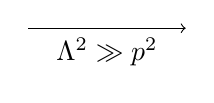
\begin{tikzpicture}
    \draw[->]        (1,-0.5)   -- (3,-0.5) node[midway,below] {\(\Lambda^2 \gg p^2\)};
    %\draw[>-Stealth] (0,0.3) -- (1,0.3);
    \end{tikzpicture}
\end{subfigure}
%\setcounter{subfigure}{3}%
\begin{subfigure}{.4\textwidth}
    \centering
    \begin{tikzpicture}
    \begin{feynman}
        \vertex[blob] (m) at (1.5, 0) {};
        \vertex at (0, 1.5) (i1);
        \vertex at (0,-1.5) (i2);
        \vertex at (1.5, 0) (a);
        \vertex at (2.3, 0) (l1) {\(\frac{g_*^2}{\Lambda^2}\)};
        \vertex at (3, 1.5) (o1);
        \vertex at (3, -1.5) (o2);
        \diagram*{
            (i1) -- [fermion] (m),
            (i2) -- [fermion] (m),
            (m) -- [fermion] (o1),
            (m) -- [fermion] (o2);
        };
    \end{feynman}
    \end{tikzpicture}
\end{subfigure}
\caption{Feynman diagrams depicting a resonant process in which the new mediator particle $\Omega$ is created (left) and the approximate description of this in an EFT, where the diagram is reduced to a four-point interaction.}
\label{fig:EFTMediatorToFourPoint}
\end{figure}
For the EFT description of this simplification to be valid, the energy involved in processes containing the effective vertex introduced by the relevant operator must thus lie well below $m_{\Omega}$, which represents the previously introduced new physics scale $\Lambda$. Practically, this can be achieved by placing an upper limit \mcut \, on the total energy that is considered in measurements of such processes. The requirement can be expressed as
\begin{align}
    \mathrm{M_{cut}} < \Lambda . 
\end{align}
\\
A good estimator of \mcut \, is the inviariant mass of the final state particles of a process. In case of the cH process, the invariant mass of the Higgs boson and jet system is a natural choice.\\
\\
The second condition that must be met is related to the perturbativity of the theory. Concretely, this means that higher dimensional operators should contribute increasingly smaller corrections so that the sum of operator contributions converges. In the case of this work where only d=6 operators are considered, this means ensuring contributions from d=8 operators and higher are sufficiently small. While this cannot be determined with certainty without explicit knowledge of the underlying theory the EFT is estimating, a popular choice is to require that at most $g_{*} \sim 4\pi$ \cite{Elias_Mir__2013}. \\
\\
These two conditions may be combined into a single, simultaneous requirement. In \cite{Elias_Mir__2013} an effective lagrangian (ignoring relevant indices for simplicity) of the general form 
\begin{align}
\mathcal{L}_{\mathrm{eff}}=\frac{\Lambda^4}{g_*^2} \mathcal{L}\left(\frac{D_\mu}{\Lambda}, \frac{g_h \phi}{\Lambda}, \frac{g_{\psi_{L, R}} \psi_{L, R}}{\Lambda^{3 / 2}}, \frac{g F_{\mu \nu}}{\Lambda^2}\right)\,
\end{align}
\\
is obtained when a single BSM coupling $g_{*}$ is introduced. This provides a prescription for the powers of the couplings and $\Lambda$ that are associated with the SM fields $\phi, \psi$ and $F_{\mu \nu}$, and the covariant derivate ${D_\mu}$. Here, $g$ represents the unaltered gauge field couplings of the SM, while $g_{\psi_{L, R}}$ and $g_h$ represent the coupling of SM fermion and the Higgs doublet to the BSM theory. In a single BSM coupling scenario, this simplifies to $g_{\psi_{L, R}} = g_h = g_*$. Applying this prescription to the CMD operator gives 

\begin{align}
    \hat{O}_{cG} \longrightarrow&
    \,\frac{\Lambda^4}{g^2_\star} \left[\left(\frac{g_\star \psi_{L,R}}{\Lambda^{3/2}}\right) \cdot \left(\frac{g_\star \psi_{L,R}}{\Lambda^{3/2}}\right) \cdot \left(\frac{g_\star \phi}{\Lambda}\right) \cdot \left(\frac{g_s G}{\Lambda^2}\right)\right] \\
    &= \frac{g_\star g_s}{\Lambda^2} \left( \psi_{L,R} \cdot \psi_{L,R}\cdot \phi \cdot G \right)\,. \label{CMDOperatorCoupling}
\end{align}
\\
Reading off from \autoref{CMDOperatorCoupling}, one can see that the coupling of the CMD operator is given by $g_\star g_s/\Lambda^2$. Comparing to \autoref{EFTEquation} thus reveals that the CMD Wilson coefficient is given by $C_{cG} = g_* g_s$. By requiring the first validity condition, the relation 

\begin{align}
    \frac{C_{cG}}{\Lambda^2} < \frac{g_* g_s}{\mathrm{M_{cut}^2}}
\end{align}
\\
is obtained. Since both $C_{cG}$ and $\Lambda$ are a priori unknown, we can redefine $\tilde{C}_{cG} = \frac{C_{cG}}{\Lambda^2}$. With this redefinition and by setting $g_{*} \sim 4\pi$, the expression

\begin{align}
      \frac{\left| \tilde{C}_{cG} \right| M_{\mathrm{cut}}^2}{4\pi g_s} < 1\,.
\end{align}
\\
can be used to define a plane in $\tilde{C}_{cG}$ and \mcut \, that satisfies the previously discussed conditions.